\begin{center}\textbf{INTRODUCTION}
\end{center}

Depuis l'apparition d'internet, il est possible de communiquer d'un bout à l'autre de la planète. Cependant, en même temps que ce dernier, sont apparus de nombreux vices, plus connus sous le nom de cybercriminalité. Face à cette menace, il s’est très vite imposé le besoin de garantir l’authenticité et l'intégrité des informations échangées sur Internet. \\
En fait, ce besoin remonte à plus loin, dès l'époque où l'Homme a été capable de communiquer. Par exemple, pendant la seconde guerre mondiale, les puissances impliquées ont dû mettre en jeu de nombreux stratagènes cryptographiques dans le but de garantir l'intégrité et l'authenticité des informations qu'elles recevaient. Dès lors, les MACs(Message Authentification Codes) se sont imposés comme une solution inncontournable pour satisfaire ce besoin. \\
Le but de cet exposé sera donc de nous permettre, futurs ingénieurs informaticiens, de comprendre le fonctionnnement des MACs et ainsi de garantir l'intégrité et l'authenticité des informations qui seront amenées à circuler dans les systèmes d'information que nous serons amenés à mettre ne place dans l'avenir.

\newpage

\section{\textbf{\underline{INTRODUCTION AU MAC}}}
\subsection{\textbf{\underline{DEFINITION DU MAC}}}

Un \textbf{code d'authentification de message}, de l'anglais Message Authentification Code, en abrégé \textbf{MAC}, est une valeur calculée à partir d'un message et d'une \textbf{clé secrète partagée entre l'émetteur et le destinataire du message}. Ce MAC est ensuite envoyé avec le message au destinataire, et le destinataire peut le vérifier en utilisant la même clé et la même fonction de calcul que l'émetteur.

Le MAC est un outil essentiel dans le domaine des correspondances secrètes en ce sens qu'il permet de garantir deux des qualités d'une bonne information (dans ce cas l'information portée par le message):
\begin{itemize}[label=$\cdot$]
    \item \textbf{L'intégrité} : En fait l'algorithme de calcul d'un MAC donne des résultats différents si on change le contenu du message, ce qui permet d'éviter en général la modification du message, et dans d'autres cas d'aviser le destinataire d'une quelconque modification de son message.
    \item \textbf{L'authenticité} : De même, il  donne des résultats différents si on change l'émetteur et/ou le destinataire du messages, ce qui permet ainsi d'éviter les usurpations d'identité.
\end{itemize}
\subsection{\textbf{\underline{FONCTIONNEMENT DU MAC}}}

Le principe de fonctionnement des MACs est plutôt simple, en ce sens qu'il s'agit pour l'émetteur :
\begin{itemize}[label=$\cdot$]
    \item D'écrire le message.
    \item De calculer son MAC à l'aide de l'algorithme de calcul et de la clé secrète qu'il a en commun avec le destinataire.
	\item D'envoyer le MAC et le message au destinataire.
\end{itemize}
Pour le destinataire:
\begin{itemize}[label=$\cdot$]
    \item Une fois le message reçu, le destinataire calcule son MAC à l'aide de la clé secrète qu'il a en commun avec l'émetteur.
    \item Il compare le résultat obtenu avec le MAC envoyé par l'émetteur: En cas d'égalité, le message est authentique et intègre, par contre, s'il est  diffèrent, il est soit corrompu soit non authentique.
\end{itemize}

\begin{center}
\textbf{Schema illustratif de la situation}:\newline \newline

    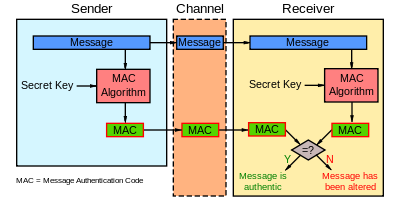
\includegraphics[width=10cm, height=5cm]{Sections/Images/fonctionnement.png}
\end{center}

Nous venons de presenter de facon generale ce qu'est le MAC, afin de faciliter la comprehension de la chose nous allons passer a une illustration.

Supposons que un général de l'armée Française veuille envoyer une demande de renforts au général de l'armée Anglaise mais ne veut pas que son message soit corrompu:

-	Il commence par écrire son message M : "Ici France, demande renforts en urgence"
-	Il calcule son MAC avec l'algorithme de calcul G et la clé secrète K\\
G(M, K) = 0101010101010001111100101001001110010 (par exemple)\\
-	Il envoie ensuite son message et son MAC au général Anglais (il peut décider de crypter son message ou  non, cela ne nous intéresse pas)
-	Le général Anglais reçoit le message et le MAC (il décrypte le message si nécessaire
-	Il recalcule le MAC à partir du message qu'il a reçu, de l'algorithme de calcul et de sa clé secrète commune avec le général Français et il le compare au MAC reçu, par exemple il reçoit M:"Ici France, demande renforts en urgence" et il calcule le MAC :\\
G(M, K) = 0101010101010001111100101001001110010\\ les MACs sont identiques, donc il peut se fier au message
Imaginons que le message ait été modifié par le général Allemand et que le général Anglais reçoit plutôt M' : "Ici France, vous les Anglais être poules mouillées, laissez nous gérer cette guerre tous seuls, bande de faibles", il calcule le MAC et obtient:\\
G(M', K) = 1100101101001011010111011001101000111 (par exemple)\\ les MACs sont différents, il sait qu'il ne peut pas se fier au message et il recherche un moyen de s'entendre avec la France sur un autre moyen de communication.

\subsection{\textbf{\underline{CHOIX DE LA CLE SECRETE}}}
Dans le contexte du code d'authentification de message (MAC), la clé secrète utilisée pour la génération et la vérification des MACs est généralement générée à l'aide d'un processus de génération de clé sécurisé. L'échange sécurisé de la clé secrète peut être réalisé à travers diverses méthodes, telles que des protocoles d'établissement de clé ou des mécanismes de distribution de clé sécurisés.

Voici un aperçu général de la génération de clé secrète et de l'échange sécurisé dans les systèmes MAC :

\begin{enumerate}
    \item \textbf{Génération de clé secrète }: La clé secrète joue un rôle essentiel dans les algorithmes MAC. Il s'agit d'un secret partagé connu uniquement des entités impliquées dans la communication.\\\\
    La clé secrète doit être générée à l'aide d'un \textbf{générateur de nombres aléatoires cryptographiquement sécurisé} (CSPRNG) pour garantir une entropie suffisante et une résistance aux attaques par force brute.\\\\
    Selon l'algorithme MAC spécifique et ses exigences, la longueur de la clé peut varier. Il est essentiel d'utiliser une longueur de clé offrant un niveau de sécurité adéquat.
    
    \item \textbf{Échange sécurisé de clé} : L'échange sécurisé de la clé secrète entre les parties communicantes est crucial pour maintenir la confidentialité et l'intégrité du MAC.\\\\
    Des protocoles d'établissement de clé, tels que l'échange de \textbf{clés Diffie-Hellman} accompagné par la \textbf{signature numérique} (pour vérifié la non répudiation), peuvent être utilisés pour établir une clé secrète partagée de manière sécurisée sur un canal non sécurisé.\\\\
    Alternativement, si les parties communicantes partagent déjà un canal sécurisé (par exemple, une connexion sécurisée préétablie ou un environnement physiquement sécurisé), elles peuvent échanger la clé secrète directement via ce canal.\\
    
    \item \textbf{Distribution de clé} : Dans certains cas, une tierce partie de confiance peut être impliquée dans la distribution sécurisée de la clé secrète aux parties communicantes.\\\\
    Des mécanismes de distribution de clé, tels que des \textbf{protocoles de gestion de clé} ou des \textbf{centres de distribution de clé}, peuvent être utilisés pour distribuer la clé secrète de manière sécurisée aux destinataires prévus.\\\\
    La tierce partie de confiance veille à ce que la clé secrète soit transmise de manière sécurisée à chaque partie sans interception ni altération.
    \newline \newline \newline
\end{enumerate}


\subsection{\textbf{\underline{Référence de cette partie}}}
\begin{center}
    \cite{wiki:mac}\\
    \cite{openclassrooms:mac}\\
    \cite{principe:mac}\\
    \cite{saied2014lightweight}\\
    \cite{dasari2015random}\\
    \cite{boumso2006methode}\\
\end{center}
